
\par As was mentioned above, the starting point of our analysis is the topic decomposition of the corpus.
We chose to decompose the corpus in 10 topics, which three of them we interpret to be talking about the same macro-topic which we called \emph{Elections}, while other two were intereted as talking about other macro-topic called \emph{Missing person}, as can be seen below. 
The meaning of the topics or macro-topics are more explained in section \ref{sec:Context}. 
So the final description of the agendas is made with only 7 topics.
We opted for choosing this arbitrary number of topics in order to describe the corpus with as least information as possible, but it is not more than an arbitrary decision, validated in some manner by our knowledge of the corpus.
After the proceedings describe in section \ref{sec:Methodology}, we construct the \textbf{Media Agenda (MA)} and the \textbf{Public Agenda (PA)}, and all their derivations, as time-dependent distributions. 

\subsection{Media and Public agenda: a qualitative approach}

\par In figure \ref{fig:all_agenda} we show a bump chart of the \textbf{MA} and the \textbf{PA} discriminated by \textbf{GT} and \textbf{Tw}. 
A bump chart is a very useful visualization tool for displaying the relative weight of the topics and at the same time their ranking, putting on the top the most important topic at a particular date.

% Global Agenda figure!!!
\begin{figure}[h]
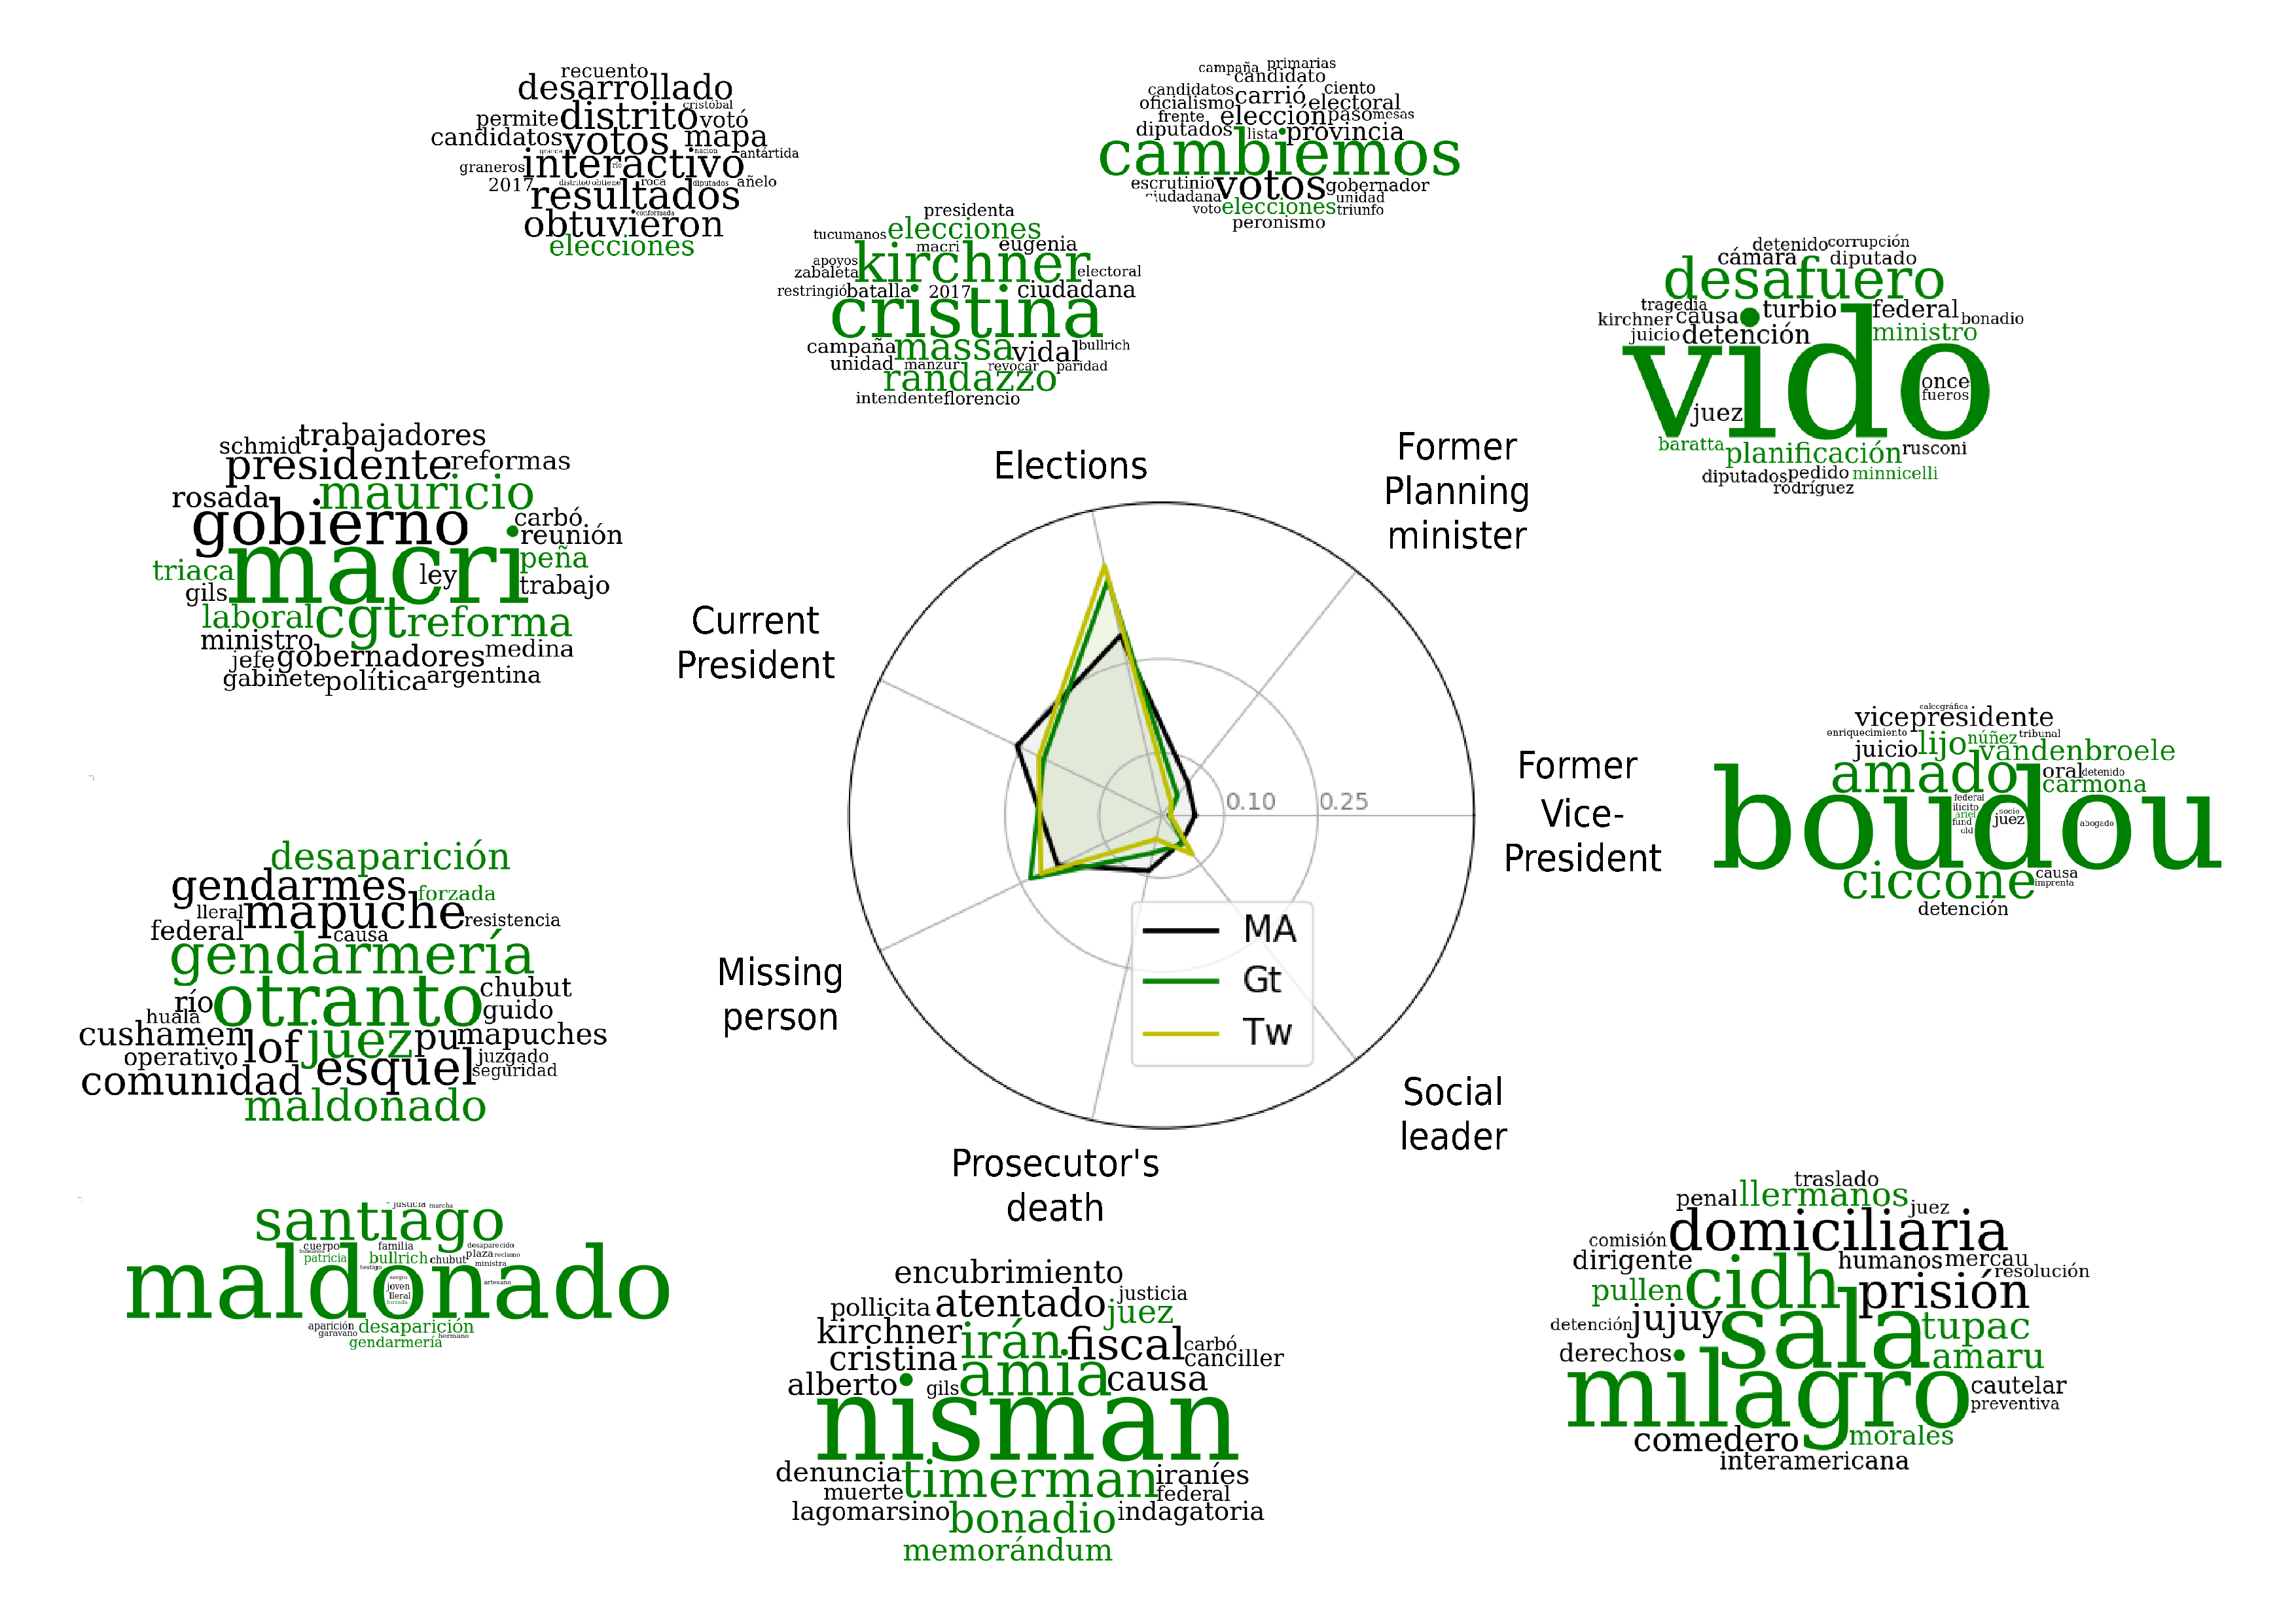
\includegraphics[width = \textwidth]{images/Fig1.pdf}
\caption{\textbf{Bump graph of the Media Agenda (MA) and Public Agenda extracted from Google Trends (Gt) and Twitter (Tw)} Topics’ names are introduced and some important events are pointed out. The curves’ width and their ordering are related to the topics’ relative weight.}
\label{fig:all_agenda}
\end{figure}
 
The topics' names are introduced in the figure, where we also point out some important events related to them.
\par In figure \ref{fig:topics_wordclouds}, we show the wordclouds of the keywords that define each topic, where the size of the word belongs to the importance in the topic's definition given by the topic detection algorithm. In green color, we point out the words involved in the Google Trends and Twitter queries in order to construct the Public Agenda. The queries employed are also specified in table \ref{table:gt_all_correlation} together with the linear correlation between the topics' temporal profiles that form the Public Agenda and their counterparts in the Media Agenda.

\footnote{Due to different characteristics in the search tool of Twitter, we adapted the queries employed here but preserving the at least at we can the most important keywords. The queries employed by topic were: \\
Elections: elecciones + cambiemos + kirchner + massa + randazzo \\
Missing person: maldonado + otranto + gendarmeria + desaparicion \\
Former Planning minister: vido + desafuero + minnicelli + baratta \\
Current President: macri + cgt + laboral +  triaca \\
Social leader:  sala + cidh + tupac + amaru + pullen + llermanos + morales \\
Prosecutor’s death: nisman + amia + memorandum + timerman +  bonadio \\
Former Vice-President:  boudou + ciccone +  lijo + vandenbroele + carmona
}

\par In figure \ref{fig:topics_wordclouds}, we also show the radar plots of the distributions made up by averaging over time the Agendas of figure \ref{fig:all_agenda}, as a way to reduce that information which would help in farther discussions. We use radar plots as an alternative of histograms because its facility in distributions comparison.  

% Wordclouds
\begin{figure}[h]
\centering
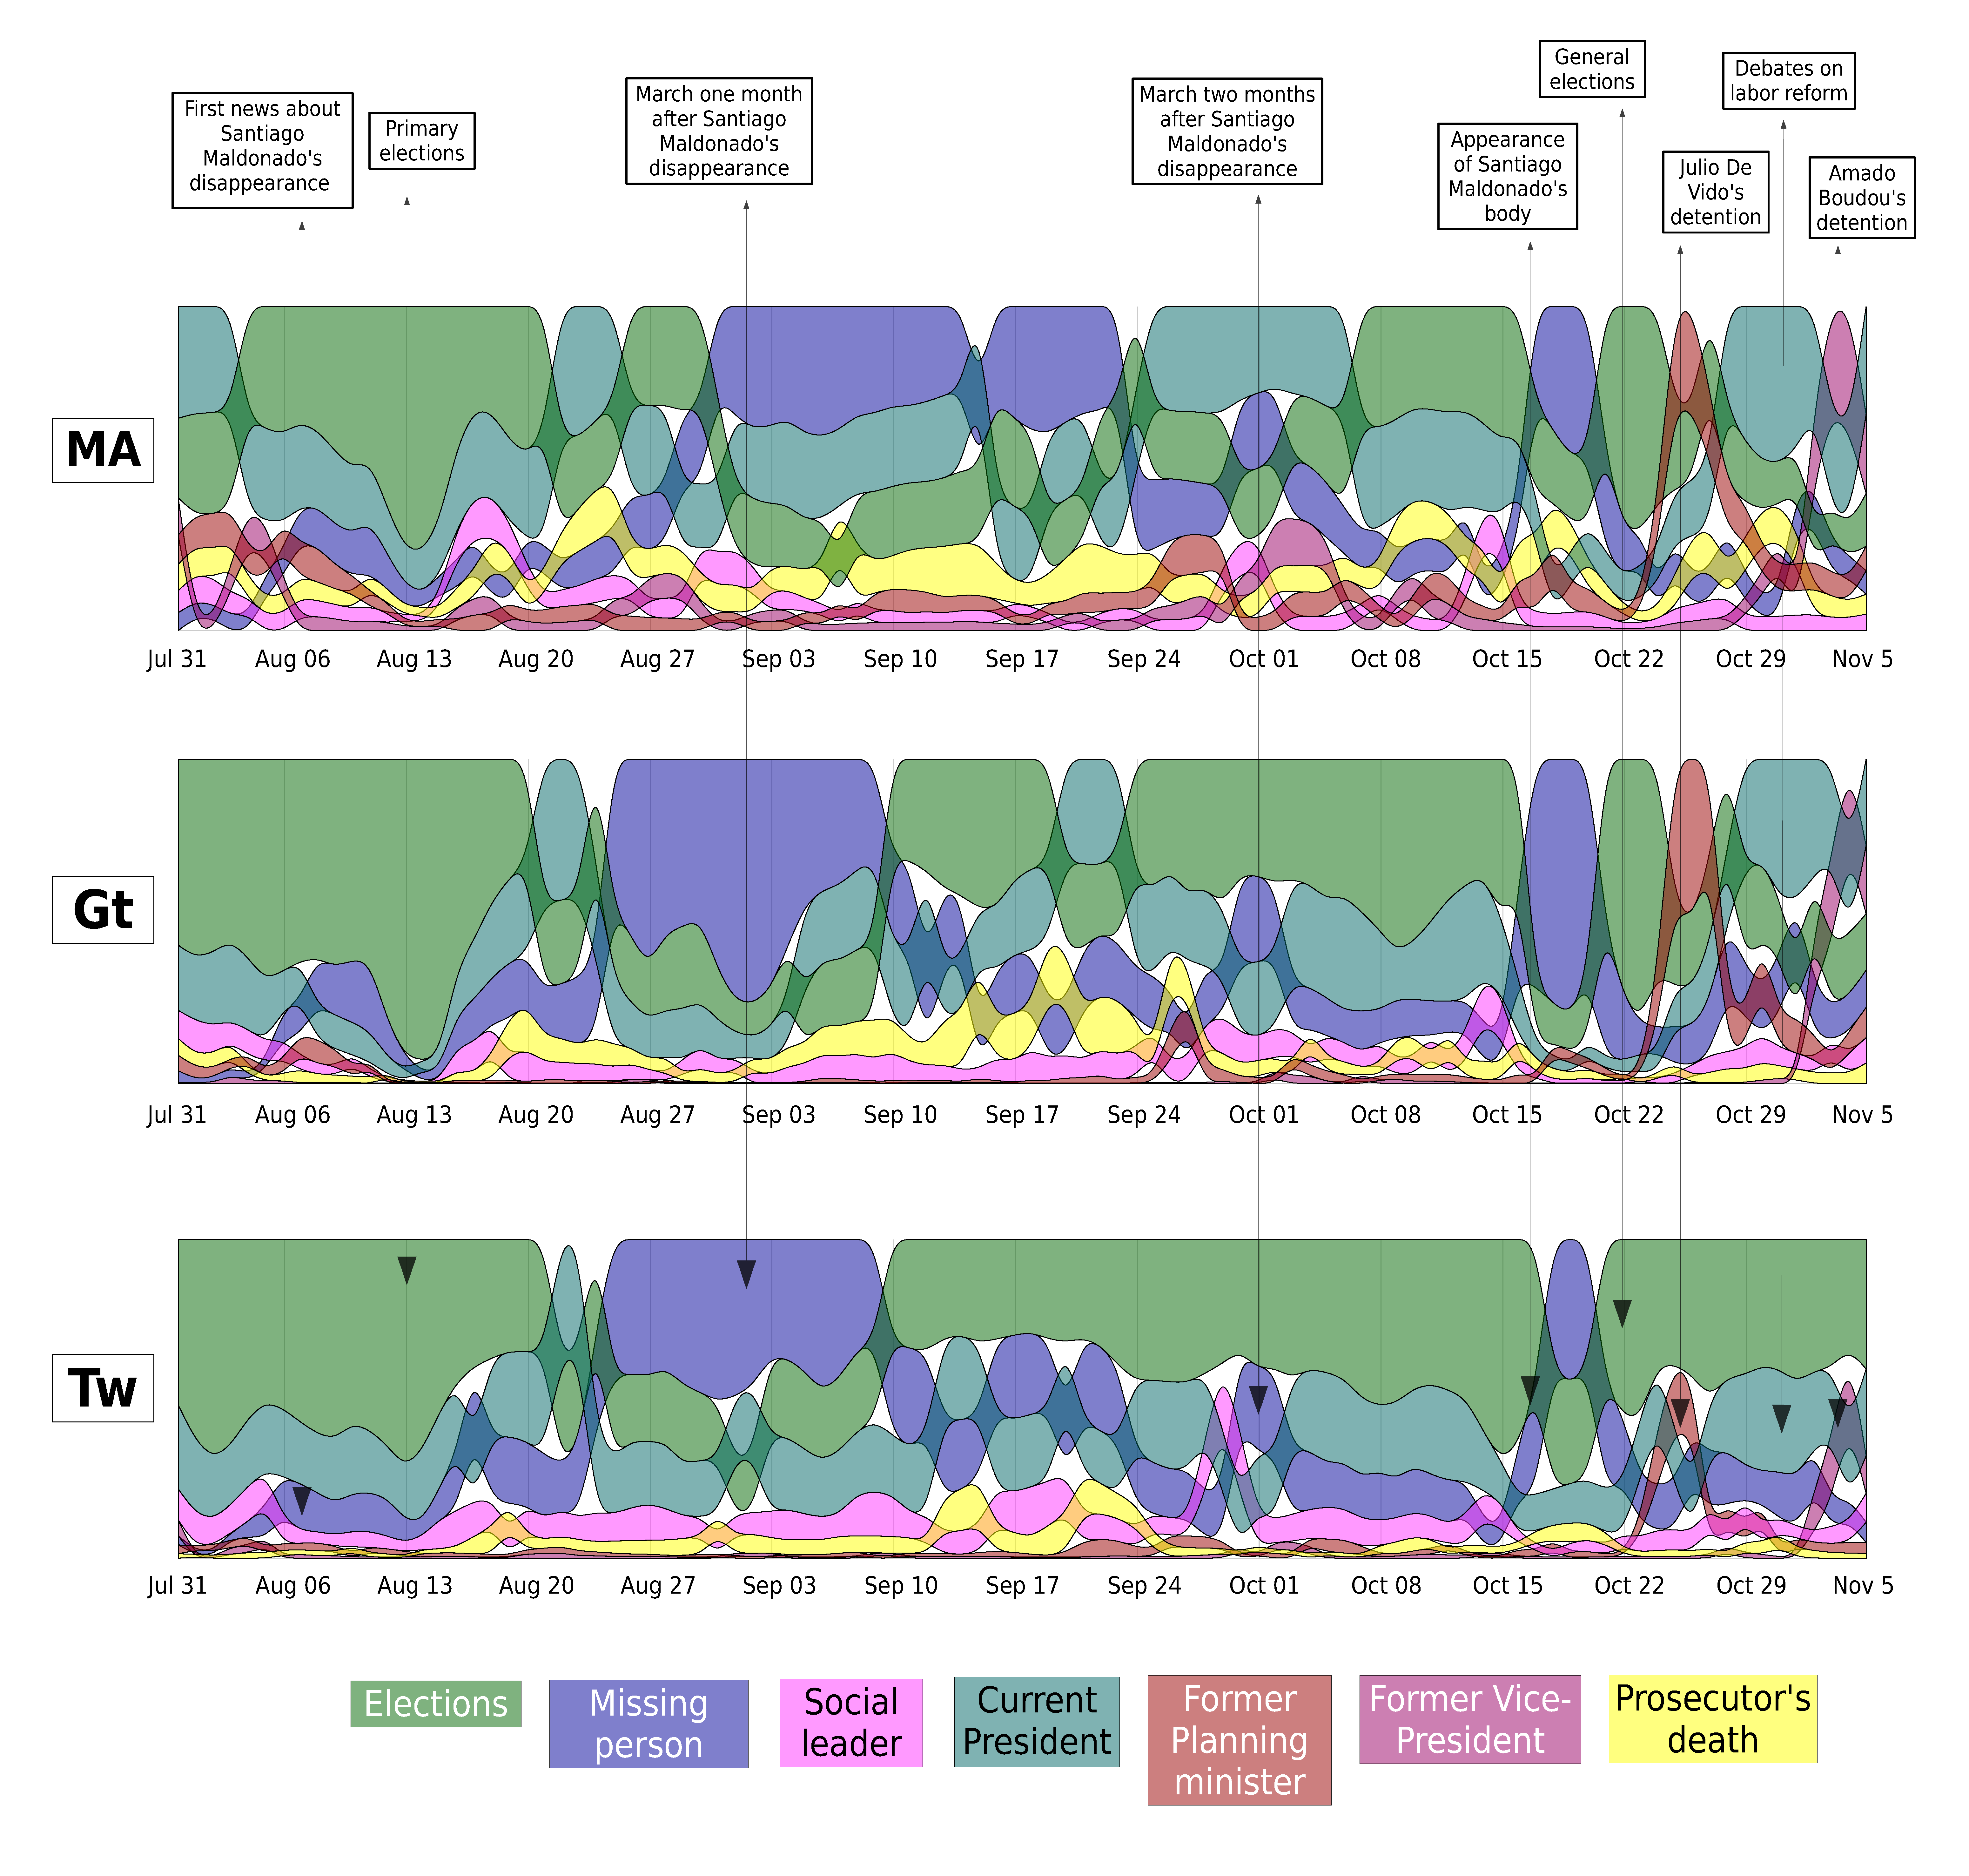
\includegraphics[width = \textwidth]{images/Fig2.pdf}
\caption{\textbf{Wordclouds and radar plot of Media and Public Agenda as an average distribution.}
In the last one, it can be seen, for instance, a greater interest of the audience in the topic Missing person than the Media. 
The wordclouds show the most important keywords involved in the definition of each topic, where in green color we show those included in the Google Trends and Twitter queries (see table \ref{table:gt_all_correlation}) and therefore in our construction of the Public Agenda.
}
\label{fig:topics_wordclouds}
\end{figure}

% Table with queries and correlations
\begin{table}[h]
\centering
\resizebox{\textwidth}{!}{\begin{tabular}{llccc}
\toprule
& Google Trends query & Correlation MA and Gt & MA and Twitter & Gt and Twitter \\ 
\midrule
Elections & elecciones + cambiemos + cristina kirchner + massa + randazzo & \textbf{0.81} & \textbf{0.59} & \textbf{0.75} \\
Missing person & santiago maldonado + juez otranto + patricia bullrich + gendarmería + desaparición forzada & \textbf{0.68} & \textbf{0.76} & \textbf{0.89} \\
Former Planning minister & de vido + desafuero + ministro de planificación + minnicelli + baratta & \textbf{0.92} & \textbf{0.82} & \textbf{0.87} \\
Current President & mauricio macri + cgt + reforma laboral + peña + triaca & \textbf{0.77} & \textbf{0.75} & \textbf{0.63} \\
Social leader & milagro sala + cidh + tupac amaru + pullen llermanos + morales & \textbf{0.49} & \textbf{0.25(*)} & \textbf{0.57} \\
Prosecutor's death & nisman + amia + memorándum con irán + timerman + juez bonadio & \textbf{0.56} & \textbf{0.59} & \textbf{0.75} \\
Former Vice-President & amado boudou + ciccone + ariel lijo + vandenbroele + núñez carmona & \textbf{0.90} & \textbf{0.92} & \textbf{0.97}\\
\bottomrule
\end{tabular}}


\caption{Queries performed in Google Trends in order to made up the Public Agenda. 
We also shown the correlation between the topics' temporal profiles of the Public Agenda and their counterpart in Media Agenda.
All correlation values are statistical significant ($p < 10^{-9}$), except (*) which is significant with $p < 0.05$.}
\label{table:gt_all_correlation}
\end{table}


\par The figures introduced above show in a qualitative way the differences between the agendas, and the dynamics of the topics, i.e. the range of dates in which a given topic was an important one, for which topic it was replaced, and so on. 
We can see, for instance in the radar plot of figure \ref{fig:topics_wordclouds}, a more interest of the audience in the topic \emph{Missing person} than the Media, or inversely in the topic \emph{Prosecutor's death}, when we see all the period analyzed as a whole. 
Also we can observe a great similarity between \textbf{Gt} and \textbf{Tw} agendas which form the Public Agenda.
\par On the other hand, the linear correlations of table \ref{table:gt_all_correlation} are in all cases positive and statistically significant, which we interpret as a form of validation of the topics found in the corpus and the keywords that describe it. 
We expected that the Media's and public's interest should generally follow a similar a pattern due to the external events, although the periods where those differ are of particular interest for us. 
A non positive (or a non significant) correlation may imply that we are not properly detecting the keywords or features that describe a particular topic, so the Google Trends' or Twitter's pattern would not be able to reflect a similar behavior that its counterpart in the Media.

% Temporal_profiles
\begin{figure}[h]
\centering
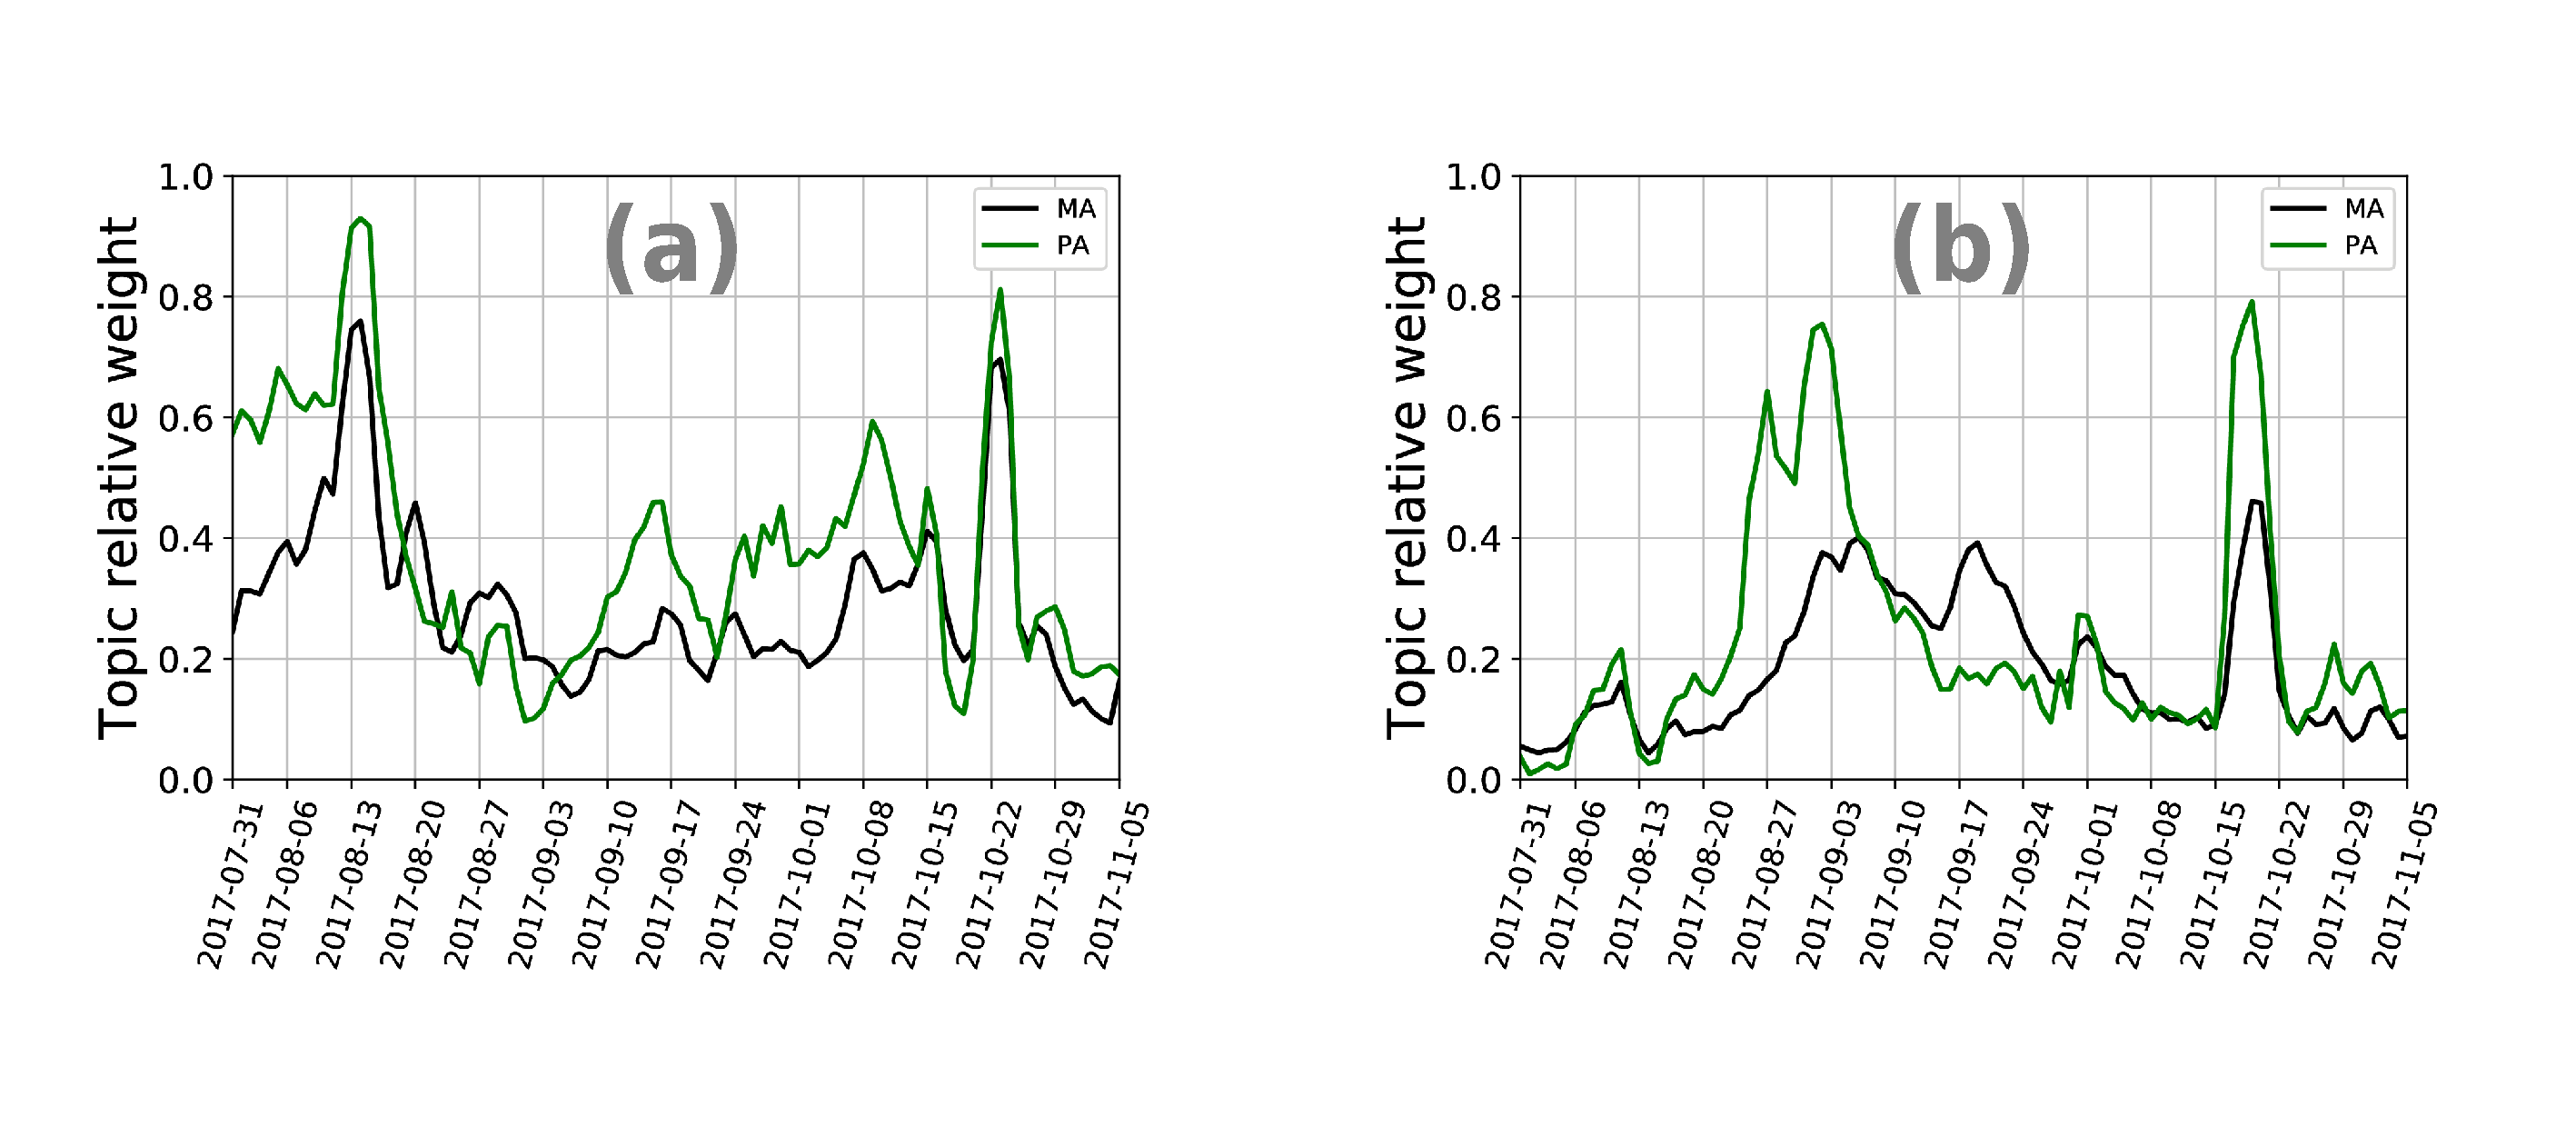
\includegraphics[width = \textwidth]{images/Fig2_5.pdf}
\caption{\textbf{AUXILIAR IMAGE: Temporal profiles.}
Elections (left) and Missing Person (right).
}
\end{figure}
